% %NOTE:
% % CHECKED WITH SLIDES: YES!
% % CHECKED WITH EXERCISES: NO -- TODO
% % MISSING: nothing :)

\section{Resource sharing}

\subsection{Terms}
\begin{definition}[Mutual Exclusion]
The requirement of ensuring that no two concurrent processes are in their critical section at the same time; it is a basic requirement in concurrency control, to prevent race conditions.
\end{definition}

\begin{definition}[Critical section]
A piece of code executed under mutual exclusion constraints.
\end{definition}

\begin{definition}[Blocked]
A task waiting for an exclusive resource.
\end{definition}


\begin{figure}[ht]
	\centering
  	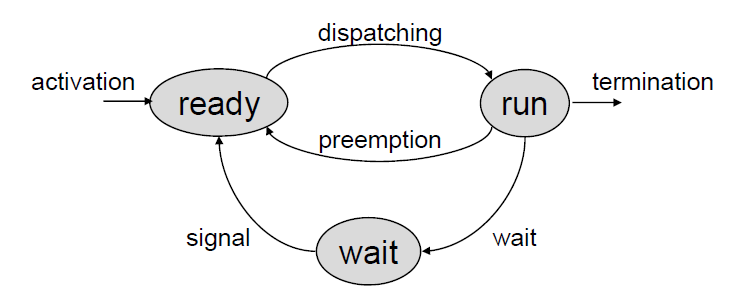
\includegraphics[scale=0.3]{img/5_resource_run_cycle.png}
	\caption{By preemption of the lock-holder, the blocked process goes into the ready pool. There it is decided, which thread to run next.}
	\label{fig1}
\end{figure}


\subsection{Solutions to Resource Sharing}

\begin{itemize}[noitemsep]
\item Non-preemptive tasks
\item Disable interrupts
\item Static scheduling
\item Use of semaphores
\end{itemize}



\subsection{Priority Inversion}

\subsubsection{Problem}
A task with a middle priority $J_2$ can get the CPU for an arbitrary time, although a task with highest priority $J_1$ is waiting, caused by the lockholder $J_3$ with lowest priority!

\begin{figure}[ht]
	\centering
  	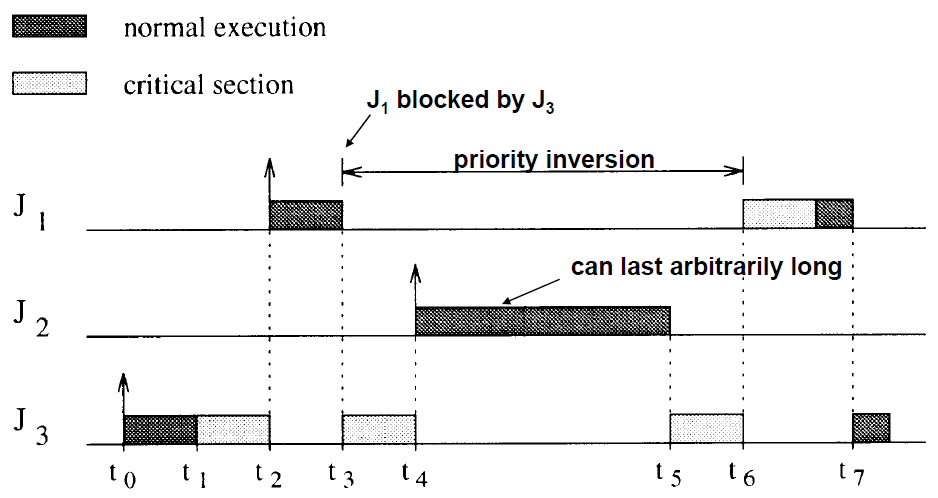
\includegraphics[scale=0.35]{img/5_resource_priority_inversion_1.png}
	\caption{Example of priority inversion}
	\label{fig2}
\end{figure}


\subsubsection{Solution - Disallow preemption}
Disallow preemption during the execution of all critical
sections. Simple, but creates unnecessary blocking as
unrelated tasks may be blocked. Deadlines now must become longer.

\subsubsection{Solution - Priority Inheritance Protocol (PIP)}
Idea: Modify the priority of those tasks that cause
blocking. When a task $J_i$ blocks one or more higher priority
tasks, it temporarily assumes a higher priority.
\\\\
Assumption:
\begin{itemize}[noitemsep]
\item n tasks which cooperate through m shared resources
\item fixed priorities
\end{itemize}

Algorithm:

\begin{enumerate}[noitemsep]
\item Jobs are scheduled based on their active priorities. Jobs with the 
same priority are executed in a FCFS discipline.
\item When a job $J_i$ tries to enter a critical section and the resource is
blocked by a lower priority job, the job $J_i$ is blocked.
\item When a job $J_i$ is blocked, it transmits its active priority to the job $J_k$
that holds the semaphore. $J_k$ resumes and executes the rest of its
critical section with a priority $p_k=p_i$
\item When $J_k$ exits a critical section, it unlocks the semaphore and the
highest priority job blocked on that semaphore is awakened. If no
other jobs are blocked by $J_k$, then $p_k$ is set to $P_k$, otherwise it is set to
the highest priority of the jobs blocked by $J_k$.
\item Priority inheritance is transitive
\end{enumerate}

Deadlock can still occur, for example when the following is executed with $J_2$ higher priority than $J_1$:
$J_1$: wait($S_a$); - $J_2$: wait($S_b$); wait($S_a$); - $J_1$: wait($S_b$);

\cleardoublepage